\documentclass[1p]{elsarticle_modified}
%\bibliographystyle{elsarticle-num}

%\usepackage[colorlinks]{hyperref}
%\usepackage{abbrmath_seonhwa} %\Abb, \Ascr, \Acal ,\Abf, \Afrak
\usepackage{amsfonts}
\usepackage{amssymb}
\usepackage{amsmath}
\usepackage{amsthm}
\usepackage{scalefnt}
\usepackage{amsbsy}
\usepackage{kotex}
\usepackage{caption}
\usepackage{subfig}
\usepackage{color}
\usepackage{graphicx}
\usepackage{xcolor} %% white, black, red, green, blue, cyan, magenta, yellow
\usepackage{float}
\usepackage{setspace}
\usepackage{hyperref}

\usepackage{tikz}
\usetikzlibrary{arrows}

\usepackage{multirow}
\usepackage{array} % fixed length table
\usepackage{hhline}

%%%%%%%%%%%%%%%%%%%%%
\makeatletter
\renewcommand*\env@matrix[1][\arraystretch]{%
	\edef\arraystretch{#1}%
	\hskip -\arraycolsep
	\let\@ifnextchar\new@ifnextchar
	\array{*\c@MaxMatrixCols c}}
\makeatother %https://tex.stackexchange.com/questions/14071/how-can-i-increase-the-line-spacing-in-a-matrix
%%%%%%%%%%%%%%%

\usepackage[normalem]{ulem}

\newcommand{\msout}[1]{\ifmmode\text{\sout{\ensuremath{#1}}}\else\sout{#1}\fi}
%SOURCE: \msout is \stkout macro in https://tex.stackexchange.com/questions/20609/strikeout-in-math-mode

\newcommand{\cancel}[1]{
	\ifmmode
	{\color{red}\msout{#1}}
	\else
	{\color{red}\sout{#1}}
	\fi
}

\newcommand{\add}[1]{
	{\color{blue}\uwave{#1}}
}

\newcommand{\replace}[2]{
	\ifmmode
	{\color{red}\msout{#1}}{\color{blue}\uwave{#2}}
	\else
	{\color{red}\sout{#1}}{\color{blue}\uwave{#2}}
	\fi
}

\newcommand{\Sol}{\mathcal{S}} %segment
\newcommand{\D}{D} %diagram
\newcommand{\A}{\mathcal{A}} %arc


%%%%%%%%%%%%%%%%%%%%%%%%%%%%%5 test

\def\sl{\operatorname{\textup{SL}}(2,\Cbb)}
\def\psl{\operatorname{\textup{PSL}}(2,\Cbb)}
\def\quan{\mkern 1mu \triangleright \mkern 1mu}

\theoremstyle{definition}
\newtheorem{thm}{Theorem}[section]
\newtheorem{prop}[thm]{Proposition}
\newtheorem{lem}[thm]{Lemma}
\newtheorem{ques}[thm]{Question}
\newtheorem{cor}[thm]{Corollary}
\newtheorem{defn}[thm]{Definition}
\newtheorem{exam}[thm]{Example}
\newtheorem{rmk}[thm]{Remark}
\newtheorem{alg}[thm]{Algorithm}

\newcommand{\I}{\sqrt{-1}}
\begin{document}

%\begin{frontmatter}
%
%\title{Boundary parabolic representations of knots up to 8 crossings}
%
%%% Group authors per affiliation:
%\author{Yunhi Cho} 
%\address{Department of Mathematics, University of Seoul, Seoul, Korea}
%\ead{yhcho@uos.ac.kr}
%
%
%\author{Seonhwa Kim} %\fnref{s_kim}}
%\address{Center for Geometry and Physics, Institute for Basic Science, Pohang, 37673, Korea}
%\ead{ryeona17@ibs.re.kr}
%
%\author{Hyuk Kim}
%\address{Department of Mathematical Sciences, Seoul National University, Seoul 08826, Korea}
%\ead{hyukkim@snu.ac.kr}
%
%\author{Seokbeom Yoon}
%\address{Department of Mathematical Sciences, Seoul National University, Seoul, 08826,  Korea}
%\ead{sbyoon15@snu.ac.kr}
%
%\begin{abstract}
%We find all boundary parabolic representation of knots up to 8 crossings.
%
%\end{abstract}
%\begin{keyword}
%    \MSC[2010] 57M25 
%\end{keyword}
%
%\end{frontmatter}

%\linenumbers
%\tableofcontents
%
\newcommand\colored[1]{\textcolor{white}{\rule[-0.35ex]{0.8em}{1.4ex}}\kern-0.8em\color{red} #1}%
%\newcommand\colored[1]{\textcolor{white}{ #1}\kern-2.17ex	\textcolor{white}{ #1}\kern-1.81ex	\textcolor{white}{ #1}\kern-2.15ex\color{red}#1	}

{\Large $\underline{12a_{0379}~(K12a_{0379})}$}

\setlength{\tabcolsep}{10pt}
\renewcommand{\arraystretch}{1.6}
\vspace{1cm}\begin{tabular}{m{100pt}>{\centering\arraybackslash}m{274pt}}
\multirow{5}{120pt}{
	\centering
	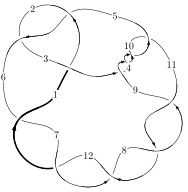
\includegraphics[width=112pt]{../../../GIT/diagram.site/Diagrams/png/1180_12a_0379.png}\\
\ \ \ A knot diagram\footnotemark}&
\allowdisplaybreaks
\textbf{Linearized knot diagam} \\
\cline{2-2}
 &
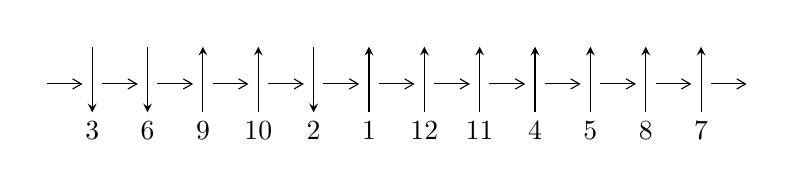
\begin{tikzpicture}[x=20pt, y=17pt]
	% nodes
	\node (C0) at (0, 0) {};
	\node (C1) at (1, 0) {};
	\node (C1U) at (1, +1) {};
	\node (C1D) at (1, -1) {3};

	\node (C2) at (2, 0) {};
	\node (C2U) at (2, +1) {};
	\node (C2D) at (2, -1) {6};

	\node (C3) at (3, 0) {};
	\node (C3U) at (3, +1) {};
	\node (C3D) at (3, -1) {9};

	\node (C4) at (4, 0) {};
	\node (C4U) at (4, +1) {};
	\node (C4D) at (4, -1) {10};

	\node (C5) at (5, 0) {};
	\node (C5U) at (5, +1) {};
	\node (C5D) at (5, -1) {2};

	\node (C6) at (6, 0) {};
	\node (C6U) at (6, +1) {};
	\node (C6D) at (6, -1) {1};

	\node (C7) at (7, 0) {};
	\node (C7U) at (7, +1) {};
	\node (C7D) at (7, -1) {12};

	\node (C8) at (8, 0) {};
	\node (C8U) at (8, +1) {};
	\node (C8D) at (8, -1) {11};

	\node (C9) at (9, 0) {};
	\node (C9U) at (9, +1) {};
	\node (C9D) at (9, -1) {4};

	\node (C10) at (10, 0) {};
	\node (C10U) at (10, +1) {};
	\node (C10D) at (10, -1) {5};

	\node (C11) at (11, 0) {};
	\node (C11U) at (11, +1) {};
	\node (C11D) at (11, -1) {8};

	\node (C12) at (12, 0) {};
	\node (C12U) at (12, +1) {};
	\node (C12D) at (12, -1) {7};
	\node (C13) at (13, 0) {};

	% arrows
	\draw[->,>={angle 60}]
	(C0) edge (C1) (C1) edge (C2) (C2) edge (C3) (C3) edge (C4) (C4) edge (C5) (C5) edge (C6) (C6) edge (C7) (C7) edge (C8) (C8) edge (C9) (C9) edge (C10) (C10) edge (C11) (C11) edge (C12) (C12) edge (C13) ;	\draw[->,>=stealth]
	(C1U) edge (C1D) (C2U) edge (C2D) (C3D) edge (C3U) (C4D) edge (C4U) (C5U) edge (C5D) (C6D) edge (C6U) (C7D) edge (C7U) (C8D) edge (C8U) (C9D) edge (C9U) (C10D) edge (C10U) (C11D) edge (C11U) (C12D) edge (C12U) ;
	\end{tikzpicture} \\
\hhline{~~} \\& 
\textbf{Solving Sequence} \\ \cline{2-2} 
 &
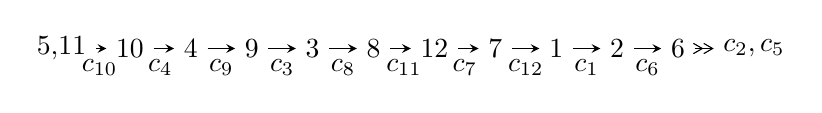
\begin{tikzpicture}[x=22pt, y=7pt]
	% node
	\node (A0) at (-1/8, 0) {5,11};
	\node (A1) at (1, 0) {10};
	\node (A2) at (2, 0) {4};
	\node (A3) at (3, 0) {9};
	\node (A4) at (4, 0) {3};
	\node (A5) at (5, 0) {8};
	\node (A6) at (6, 0) {12};
	\node (A7) at (7, 0) {7};
	\node (A8) at (8, 0) {1};
	\node (A9) at (9, 0) {2};
	\node (A10) at (10, 0) {6};
	\node (C1) at (1/2, -1) {$c_{10}$};
	\node (C2) at (3/2, -1) {$c_{4}$};
	\node (C3) at (5/2, -1) {$c_{9}$};
	\node (C4) at (7/2, -1) {$c_{3}$};
	\node (C5) at (9/2, -1) {$c_{8}$};
	\node (C6) at (11/2, -1) {$c_{11}$};
	\node (C7) at (13/2, -1) {$c_{7}$};
	\node (C8) at (15/2, -1) {$c_{12}$};
	\node (C9) at (17/2, -1) {$c_{1}$};
	\node (C10) at (19/2, -1) {$c_{6}$};
	\node (A11) at (45/4, 0) {$c_{2},c_{5}$};

	% edge
	\draw[->,>=stealth]	
	(A0) edge (A1) (A1) edge (A2) (A2) edge (A3) (A3) edge (A4) (A4) edge (A5) (A5) edge (A6) (A6) edge (A7) (A7) edge (A8) (A8) edge (A9) (A9) edge (A10) ;
	\draw[->>,>={angle 60}]	
	(A10) edge (A11);
\end{tikzpicture} \\ 

\end{tabular} \\

\footnotetext{
The image of knot diagram is generated by the software ``\textbf{Draw programme}" developed by Andrew Bartholomew(\url{http://www.layer8.co.uk/maths/draw/index.htm\#Running-draw}), where we modified some parts for our purpose(\url{https://github.com/CATsTAILs/LinksPainter}).
}\phantom \\ \newline 
\centering \textbf{Ideals for irreducible components\footnotemark of $X_{\text{par}}$} 
 
\begin{align*}
I^u_{1}&=\langle 
u^{35}- u^{34}+\cdots+3 u^2-1\rangle \\
\\
\end{align*}
\raggedright * 1 irreducible components of $\dim_{\mathbb{C}}=0$, with total 35 representations.\\
\footnotetext{All coefficients of polynomials are rational numbers. But the coefficients are sometimes approximated in decimal forms when there is not enough margin.}
\newpage
\renewcommand{\arraystretch}{1}
\centering \section*{I. $I^u_{1}= \langle u^{35}- u^{34}+\cdots+3 u^2-1 \rangle$}
\flushleft \textbf{(i) Arc colorings}\\
\begin{tabular}{m{7pt} m{180pt} m{7pt} m{180pt} }
\flushright $a_{5}=$&$\begin{pmatrix}0\\u\end{pmatrix}$ \\
\flushright $a_{11}=$&$\begin{pmatrix}1\\0\end{pmatrix}$ \\
\flushright $a_{10}=$&$\begin{pmatrix}1\\u^2\end{pmatrix}$ \\
\flushright $a_{4}=$&$\begin{pmatrix}- u\\- u^3+u\end{pmatrix}$ \\
\flushright $a_{9}=$&$\begin{pmatrix}- u^2+1\\- u^4+2 u^2\end{pmatrix}$ \\
\flushright $a_{3}=$&$\begin{pmatrix}u^3-2 u\\u^5-3 u^3+u\end{pmatrix}$ \\
\flushright $a_{8}=$&$\begin{pmatrix}u^4-3 u^2+1\\- u^4+2 u^2\end{pmatrix}$ \\
\flushright $a_{12}=$&$\begin{pmatrix}u^8-5 u^6+7 u^4-2 u^2+1\\- u^8+4 u^6-4 u^4\end{pmatrix}$ \\
\flushright $a_{7}=$&$\begin{pmatrix}u^{12}-7 u^{10}+17 u^8-16 u^6+6 u^4-5 u^2+1\\- u^{12}+6 u^{10}-12 u^8+8 u^6- u^4+2 u^2\end{pmatrix}$ \\
\flushright $a_{1}=$&$\begin{pmatrix}u^{16}-9 u^{14}+31 u^{12}-50 u^{10}+39 u^8-22 u^6+18 u^4-4 u^2+1\\- u^{16}+8 u^{14}-24 u^{12}+32 u^{10}-18 u^8+8 u^6-8 u^4\end{pmatrix}$ \\
\flushright $a_{2}=$&$\begin{pmatrix}u^{24}-13 u^{22}+\cdots-6 u^2+1\\u^{26}-14 u^{24}+\cdots-18 u^4+u^2\end{pmatrix}$ \\
\flushright $a_{6}=$&$\begin{pmatrix}u^{20}-11 u^{18}+\cdots-7 u^2+1\\- u^{20}+10 u^{18}+\cdots- u^4+2 u^2\end{pmatrix}$\\&\end{tabular}
\flushleft \textbf{(ii) Obstruction class $= -1$}\\~\\
\flushleft \textbf{(iii) Cusp Shapes $= -4 u^{32}+68 u^{30}+4 u^{29}-508 u^{28}-64 u^{27}+2184 u^{26}+444 u^{25}-5960 u^{24}-1744 u^{23}+10836 u^{22}+4264 u^{21}-13756 u^{20}-6804 u^{19}+13416 u^{18}+7508 u^{17}-11532 u^{16}-6528 u^{15}+8700 u^{14}+5128 u^{13}-5028 u^{12}-3288 u^{11}+2552 u^{10}+1528 u^9-1288 u^8-704 u^7+328 u^6+240 u^5-120 u^4-44 u^3+16 u^2+20 u+6$}\\~\\
\newpage\renewcommand{\arraystretch}{1}
\flushleft \textbf{(iv) u-Polynomials at the component}\newline \\
\begin{tabular}{m{50pt}|m{274pt}}
Crossings & \hspace{64pt}u-Polynomials at each crossing \\
\hline $$\begin{aligned}c_{1}\end{aligned}$$&$\begin{aligned}
&u^{35}+21 u^{34}+\cdots+6 u+1
\end{aligned}$\\
\hline $$\begin{aligned}c_{2},c_{5}\end{aligned}$$&$\begin{aligned}
&u^{35}+u^{34}+\cdots+3 u^2-1
\end{aligned}$\\
\hline $$\begin{aligned}c_{3},c_{4},c_{9}\\c_{10}\end{aligned}$$&$\begin{aligned}
&u^{35}- u^{34}+\cdots+3 u^2-1
\end{aligned}$\\
\hline $$\begin{aligned}c_{6},c_{7},c_{8}\\c_{11},c_{12}\end{aligned}$$&$\begin{aligned}
&u^{35}+3 u^{34}+\cdots+12 u+1
\end{aligned}$\\
\hline
\end{tabular}\\~\\
\newpage\renewcommand{\arraystretch}{1}
\flushleft \textbf{(v) Riley Polynomials at the component}\newline \\
\begin{tabular}{m{50pt}|m{274pt}}
Crossings & \hspace{64pt}Riley Polynomials at each crossing \\
\hline $$\begin{aligned}c_{1}\end{aligned}$$&$\begin{aligned}
&y^{35}-13 y^{34}+\cdots+10 y-1
\end{aligned}$\\
\hline $$\begin{aligned}c_{2},c_{5}\end{aligned}$$&$\begin{aligned}
&y^{35}-21 y^{34}+\cdots+6 y-1
\end{aligned}$\\
\hline $$\begin{aligned}c_{3},c_{4},c_{9}\\c_{10}\end{aligned}$$&$\begin{aligned}
&y^{35}-37 y^{34}+\cdots+6 y-1
\end{aligned}$\\
\hline $$\begin{aligned}c_{6},c_{7},c_{8}\\c_{11},c_{12}\end{aligned}$$&$\begin{aligned}
&y^{35}+47 y^{34}+\cdots+90 y-1
\end{aligned}$\\
\hline
\end{tabular}\\~\\
\newpage\flushleft \textbf{(vi) Complex Volumes and Cusp Shapes}
$$\begin{array}{c|c|c}  
\text{Solutions to }I^u_{1}& \I (\text{vol} + \sqrt{-1}CS) & \text{Cusp shape}\\
 \hline 
\begin{aligned}
u &= -0.525071 + 0.695031 I\end{aligned}
 & -15.9587 - 7.3230 I & -0.50203 + 5.74720 I \\ \hline\begin{aligned}
u &= -0.525071 - 0.695031 I\end{aligned}
 & -15.9587 + 7.3230 I & -0.50203 - 5.74720 I \\ \hline\begin{aligned}
u &= -0.503644 + 0.700836 I\end{aligned}
 & -16.0231 + 2.6486 I & -0.693389 - 0.151455 I \\ \hline\begin{aligned}
u &= -0.503644 - 0.700836 I\end{aligned}
 & -16.0231 - 2.6486 I & -0.693389 + 0.151455 I \\ \hline\begin{aligned}
u &= \phantom{-}0.512719 + 0.691106 I\end{aligned}
 & -12.06160 + 2.31682 I & \phantom{-}2.54987 - 2.83092 I \\ \hline\begin{aligned}
u &= \phantom{-}0.512719 - 0.691106 I\end{aligned}
 & -12.06160 - 2.31682 I & \phantom{-}2.54987 + 2.83092 I \\ \hline\begin{aligned}
u &= \phantom{-}0.522839 + 0.541402 I\end{aligned}
 & -5.47274 + 5.77937 I & \phantom{-}0.47146 - 7.85052 I \\ \hline\begin{aligned}
u &= \phantom{-}0.522839 - 0.541402 I\end{aligned}
 & -5.47274 - 5.77937 I & \phantom{-}0.47146 + 7.85052 I \\ \hline\begin{aligned}
u &= \phantom{-}0.408454 + 0.569281 I\end{aligned}
 & -5.82031 - 1.98611 I & -1.101715 + 0.333068 I \\ \hline\begin{aligned}
u &= \phantom{-}0.408454 - 0.569281 I\end{aligned}
 & -5.82031 + 1.98611 I & -1.101715 - 0.333068 I \\ \hline\begin{aligned}
u &= -0.459588 + 0.502405 I\end{aligned}
 & -2.40665 - 1.73767 I & \phantom{-}3.44724 + 4.36626 I \\ \hline\begin{aligned}
u &= -0.459588 - 0.502405 I\end{aligned}
 & -2.40665 + 1.73767 I & \phantom{-}3.44724 - 4.36626 I \\ \hline\begin{aligned}
u &= -0.549002 + 0.276756 I\end{aligned}
 & -0.34953 - 3.08643 I & \phantom{-}6.48319 + 9.61199 I \\ \hline\begin{aligned}
u &= -0.549002 - 0.276756 I\end{aligned}
 & -0.34953 + 3.08643 I & \phantom{-}6.48319 - 9.61199 I \\ \hline\begin{aligned}
u &= \phantom{-}1.43209\phantom{ +0.000000I}\end{aligned}
 & \phantom{-}3.32584\phantom{ +0.000000I} & \phantom{-}2.08830\phantom{ +0.000000I} \\ \hline\begin{aligned}
u &= -1.46088 + 0.14870 I\end{aligned}
 & \phantom{-}0.217823 - 0.520687 I & \phantom{-0.000000 } 0 \\ \hline\begin{aligned}
u &= -1.46088 - 0.14870 I\end{aligned}
 & \phantom{-}0.217823 + 0.520687 I & \phantom{-0.000000 } 0 \\ \hline\begin{aligned}
u &= \phantom{-}0.495921 + 0.057416 I\end{aligned}
 & \phantom{-}0.779355 + 0.040720 I & \phantom{-}13.22367 - 0.76931 I \\ \hline\begin{aligned}
u &= \phantom{-}0.495921 - 0.057416 I\end{aligned}
 & \phantom{-}0.779355 - 0.040720 I & \phantom{-}13.22367 + 0.76931 I \\ \hline\begin{aligned}
u &= \phantom{-}1.49978 + 0.13102 I\end{aligned}
 & \phantom{-}4.04258 + 3.93448 I & \phantom{-}6.00000 + 0. I\phantom{ +0.000000I} \\ \hline\begin{aligned}
u &= \phantom{-}1.49978 - 0.13102 I\end{aligned}
 & \phantom{-}4.04258 - 3.93448 I & \phantom{-}6.00000 + 0. I\phantom{ +0.000000I} \\ \hline\begin{aligned}
u &= -1.51928 + 0.02326 I\end{aligned}
 & \phantom{-}7.54181 - 0.38720 I & \phantom{-}12.42967 + 0. I\phantom{ +0.000000I} \\ \hline\begin{aligned}
u &= -1.51928 - 0.02326 I\end{aligned}
 & \phantom{-}7.54181 + 0.38720 I & \phantom{-}12.42967 + 0. I\phantom{ +0.000000I} \\ \hline\begin{aligned}
u &= -1.51926 + 0.15290 I\end{aligned}
 & \phantom{-}1.26876 - 8.24991 I & \phantom{-0.000000 -}0. + 7.12333 I \\ \hline\begin{aligned}
u &= -1.51926 - 0.15290 I\end{aligned}
 & \phantom{-}1.26876 + 8.24991 I & \phantom{-0.000000 } 0. - 7.12333 I \\ \hline\begin{aligned}
u &= \phantom{-}1.52643 + 0.06311 I\end{aligned}
 & \phantom{-}6.56659 + 4.22789 I & \phantom{-0.000000 } 0. - 6.71857 I \\ \hline\begin{aligned}
u &= \phantom{-}1.52643 - 0.06311 I\end{aligned}
 & \phantom{-}6.56659 - 4.22789 I & \phantom{-0.000000 -}0. + 6.71857 I \\ \hline\begin{aligned}
u &= \phantom{-}1.50999 + 0.23245 I\end{aligned}
 & -9.45605 + 0.74325 I & \phantom{-0.000000 } 0 \\ \hline\begin{aligned}
u &= \phantom{-}1.50999 - 0.23245 I\end{aligned}
 & -9.45605 - 0.74325 I & \phantom{-0.000000 } 0 \\ \hline\begin{aligned}
u &= -1.51605 + 0.22648 I\end{aligned}
 & -5.43016 - 5.65254 I & \phantom{-0.000000 } 0\\
 \hline 
 \end{array}$$\newpage$$\begin{array}{c|c|c}  
\text{Solutions to }I^u_{1}& \I (\text{vol} + \sqrt{-1}CS) & \text{Cusp shape}\\
 \hline 
\begin{aligned}
u &= -1.51605 - 0.22648 I\end{aligned}
 & -5.43016 + 5.65254 I & \phantom{-0.000000 } 0 \\ \hline\begin{aligned}
u &= \phantom{-}1.52333 + 0.22907 I\end{aligned}
 & -9.25340 + 10.69110 I & \phantom{-0.000000 } 0 \\ \hline\begin{aligned}
u &= \phantom{-}1.52333 - 0.22907 I\end{aligned}
 & -9.25340 - 10.69110 I & \phantom{-0.000000 } 0 \\ \hline\begin{aligned}
u &= -0.162727 + 0.381338 I\end{aligned}
 & -1.53270 + 0.77833 I & -1.99796 - 0.53208 I \\ \hline\begin{aligned}
u &= -0.162727 - 0.381338 I\end{aligned}
 & -1.53270 - 0.77833 I & -1.99796 + 0.53208 I\\
 \hline 
 \end{array}$$\newpage
\newpage\renewcommand{\arraystretch}{1}
\centering \section*{ II. u-Polynomials}
\begin{tabular}{m{50pt}|m{274pt}}
Crossings & \hspace{64pt}u-Polynomials at each crossing \\
\hline $$\begin{aligned}c_{1}\end{aligned}$$&$\begin{aligned}
&u^{35}+21 u^{34}+\cdots+6 u+1
\end{aligned}$\\
\hline $$\begin{aligned}c_{2},c_{5}\end{aligned}$$&$\begin{aligned}
&u^{35}+u^{34}+\cdots+3 u^2-1
\end{aligned}$\\
\hline $$\begin{aligned}c_{3},c_{4},c_{9}\\c_{10}\end{aligned}$$&$\begin{aligned}
&u^{35}- u^{34}+\cdots+3 u^2-1
\end{aligned}$\\
\hline $$\begin{aligned}c_{6},c_{7},c_{8}\\c_{11},c_{12}\end{aligned}$$&$\begin{aligned}
&u^{35}+3 u^{34}+\cdots+12 u+1
\end{aligned}$\\
\hline
\end{tabular}\newpage\renewcommand{\arraystretch}{1}
\centering \section*{ III. Riley Polynomials}
\begin{tabular}{m{50pt}|m{274pt}}
Crossings & \hspace{64pt}Riley Polynomials at each crossing \\
\hline $$\begin{aligned}c_{1}\end{aligned}$$&$\begin{aligned}
&y^{35}-13 y^{34}+\cdots+10 y-1
\end{aligned}$\\
\hline $$\begin{aligned}c_{2},c_{5}\end{aligned}$$&$\begin{aligned}
&y^{35}-21 y^{34}+\cdots+6 y-1
\end{aligned}$\\
\hline $$\begin{aligned}c_{3},c_{4},c_{9}\\c_{10}\end{aligned}$$&$\begin{aligned}
&y^{35}-37 y^{34}+\cdots+6 y-1
\end{aligned}$\\
\hline $$\begin{aligned}c_{6},c_{7},c_{8}\\c_{11},c_{12}\end{aligned}$$&$\begin{aligned}
&y^{35}+47 y^{34}+\cdots+90 y-1
\end{aligned}$\\
\hline
\end{tabular}
\vskip 2pc
\end{document}